% =============================================================================
%  A Lightweight Latent Mapping for Old Photo Restoration:
%  When Flow Matching Is Unnecessary
%  Standalone two-column article; port into the venue template before submission.
% =============================================================================
\documentclass[10pt,twocolumn,letterpaper]{article}
\usepackage[margin=0.75in,columnsep=0.3in]{geometry}
\usepackage{times}
\usepackage[T1]{fontenc}
\usepackage[utf8]{inputenc}
\usepackage{amsmath,amssymb,amsthm,bm}
\usepackage{graphicx}
\usepackage{booktabs}
\usepackage{multirow}
\usepackage{xcolor}
\usepackage{tikz}
\usetikzlibrary{arrows.meta,positioning,fit}
\usepackage[hidelinks]{hyperref}
\usepackage[capitalize]{cleveref}

\newtheorem{proposition}{Proposition}
\newcommand{\zA}{\bm{z}_A}
\newcommand{\zB}{\bm{z}_B}
\newcommand{\zt}{\bm{z}_t}
\newcommand{\hzB}{\hat{\bm{z}}_B}
\newcommand{\E}{\mathbb{E}}

\title{A Lightweight Latent Mapping for Old Photo Restoration:\\When Flow Matching Is Unnecessary}
\author{Mani Sankar Das}
\date{}

\begin{document}
\maketitle

% -----------------------------------------------------------------------------
\begin{abstract}
Bringing Old Photos Back to Life (BOPBTL) restores photographs by translating between the latent spaces of two frozen
variational autoencoders with a 36.1M-parameter \emph{mapping network}. We replace this mapping with a compact residual
network of 10.9M parameters, trained with BOPBTL's own loss types, and keep everything else unchanged. The mapping needs
3.3$\times$ fewer FLOPs, runs 2.1--2.9$\times$ faster on a Tesla T4 (1.7--2.5$\times$ for the full pipeline), and on an
independent 4{,}958-pair COCO benchmark recovers 86\% of BOPBTL's LPIPS improvement and 89\% of its KID improvement over
the degraded input (68\% and 71\% in a second training run). It adds as little false colour to black-and-white
photographs as BOPBTL, but is less accurate in colour and pixel fidelity and scores lower on real old photos. The
network can also be trained as a flow-matching model. We show that, for this paired problem, the flow adds nothing: a one-step flow
evaluates the network only at $t{=}0$, where its time conditioning reduces to a constant scale and shift that folds
exactly into normalisation layers, and its optimum coincides with direct regression. In a matched ablation, training
the same network along the whole flow path, with bridge noise and trajectory training, was worse than training it at
$t{=}0$ alone on every metric, and multi-step sampling added cost without improving perceptual quality.
\end{abstract}

% -----------------------------------------------------------------------------
\section{Introduction}
\label{sec:intro}

Old photographs combine structured damage (scratches, tears) with unstructured degradation (blur, film grain, fading,
compression). BOPBTL~\cite{wan2020bringing,wan2022old} handles the unstructured part with a \emph{triplet domain
translation}: a VAE encodes real old and synthetically degraded photos into a shared latent space, a second VAE encodes
clean photos, and a mapping network translates latents from the first space to the second. The mapping is trained with
a latent $\ell_1$ loss, a conditional multi-scale GAN, discriminator feature matching and a VGG perceptual
loss~\cite{wang2018pix2pixhd}. It is also the most expensive part of the global restoration stage: 36.1M parameters and
296 GFLOPs per $256{\times}256$ image, against 12.7 GFLOPs for both autoencoders together.

This paper asks a practical question: \emph{how much of BOPBTL's restoration quality does a much smaller mapping keep,
with the same frozen autoencoders and the same loss types?} Flow
matching~\cite{liu2023flow,lipman2023flow} and bridge models~\cite{liu2023i2sb,shi2023dsbm,albergo2023stochastic} are
strong tools for image-to-image translation, and the degraded latent is already close to the clean one, so a few-step
latent flow is a natural candidate. A matched ablation shows, however, that the flow adds nothing in this setting. We report both the efficient mapping and the reason the flow can be
dropped.

Our contributions are:
\begin{itemize}
  \item \textbf{A lightweight drop-in mapping for BOPBTL} (\cref{sec:method}): 10.9M parameters and 89 GFLOPs instead of
        36.1M and 296, 2.1--2.9$\times$ faster, trained with BOPBTL's loss types only, reaching 86--89\% of BOPBTL's
        LPIPS and KID improvement on COCO in our better run and 68--71\% in a second run (\cref{sec:main,sec:efficiency}).
  \item \textbf{Why a flow is unnecessary here} (\cref{sec:flow}): for paired restoration, a one-step flow reduces exactly
        to a direct network (the time conditioning folds into normalisation), and its optimum equals that of direct
        regression; in a matched ablation, flow training was worse than direct training on every metric, at one, four
        and eight sampling steps (\cref{sec:ablation}).
  \item \textbf{An evaluation that separates mapping from autoencoders}: a frozen, independent COCO benchmark with KID
        and CIEDE2000, the \emph{VAE ceiling} as an upper bound for any mapping, a colour analysis in CIELAB, and
        real-photo results, reported with the run-to-run spread (\cref{sec:exp}).
\end{itemize}

% -----------------------------------------------------------------------------
\section{Related work}
\label{sec:related}

\paragraph{Old photo restoration.} BOPBTL~\cite{wan2020bringing,wan2022old} introduced latent-space translation with two
VAEs and a mapping network, plus scratch detection and face enhancement stages. We keep its global restoration stage in
quality mode and replace only the mapping.

\paragraph{Flows and bridges for restoration.} Rectified flow~\cite{liu2023flow} and flow matching~\cite{lipman2023flow}
learn velocity fields along simple interpolation paths between two distributions. For paired image-to-image problems,
bridge models~\cite{liu2023i2sb,shi2023dsbm,albergo2023stochastic} start from the degraded sample instead of noise, as do
residual-shifting and direct-iteration methods~\cite{yue2023resshift,delbracio2023indi}; consistency
models~\cite{song2023consistency} target few-step generation. These methods transport one distribution to another and
construct the coupling between them; \cref{sec:flow} argues that in paired latent restoration this coupling is already
given, which removes the reason to use them.

\paragraph{Perception and distortion.} Pixel fidelity and perceptual quality trade off~\cite{blau2018perception}. We
therefore report PSNR, SSIM~\cite{wang2004ssim}, LPIPS~\cite{zhang2018lpips}, FID~\cite{heusel2017fid} and
KID~\cite{binkowski2018kid}, plus CIEDE2000~\cite{sharma2005ciede2000} for colour, and use none of them as a training loss.

% -----------------------------------------------------------------------------
\section{Method}
\label{sec:method}

\begin{figure}[t]
\centering
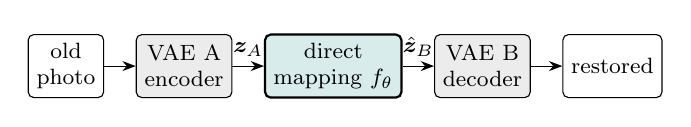
\begin{tikzpicture}[font=\footnotesize, node distance=4mm,
  box/.style={draw, rounded corners=2pt, align=center, minimum height=8mm, inner sep=3pt},
  frozen/.style={box, fill=gray!15},
  ours/.style={box, fill=teal!15, thick}]
  \node[box] (x) {old\\photo};
  \node[frozen, right=of x] (ea) {VAE A\\encoder};
  \node[ours, right=of ea] (m) {direct\\mapping $f_\theta$};
  \node[frozen, right=of m] (db) {VAE B\\decoder};
  \node[box, right=of db] (y) {restored};
  \draw[-{Stealth}] (x) -- (ea);
  \draw[-{Stealth}] (ea) -- node[above]{$\zA$} (m);
  \draw[-{Stealth}] (m) -- node[above]{$\hzB$} (db);
  \draw[-{Stealth}] (db) -- (y);
\end{tikzpicture}
\caption{Pipeline. The two VAEs of BOPBTL's global restoration stage are frozen; only the mapping is replaced, and it
runs once per image.}
\label{fig:pipeline}
\end{figure}

\subsection{Setting}
Let $E_A$ be the frozen encoder for degraded photos and $D_B$ the frozen decoder for clean photos (\cref{fig:pipeline}).
For a degraded/clean pair $(\bm{x}_A,\bm{x}_B)$ let $\zA=E_A(\bm{x}_A)$ and $\zB=E_B(\bm{x}_B)$, both 64-channel latents at
a quarter of the image resolution. We divide latents by $s$, the standard deviation of $\zB$ on held-out data.

\subsection{Architecture}
\label{sec:arch}
The mapping is residual,
\begin{equation}
  \hzB=s\,\big(\bm{a}+f_\theta(\bm{a})\big),\qquad \bm{a}=\zA/s ,
  \label{eq:mapping}
\end{equation}
so that it starts from the identity: $f_\theta$ is a $3{\times}3$ convolution to 256 channels, nine residual blocks and a
zero-initialised $3{\times}3$ output convolution. Each block computes
$\bm{h}\leftarrow\bm{h}+\mathrm{Conv}\big(\mathrm{Drop}(\mathrm{SiLU}(\mathrm{GN}(\mathrm{Conv}_d(\mathrm{SiLU}(\mathrm{GN}(\bm{h}))))))\big)$
with GroupNorm (8 groups), a dilated $3{\times}3$ convolution whose dilation $d$ cycles through 1, 2, 4 for a large
receptive field at low cost, and dropout 0.1. The network has 10.9M parameters and needs 89 GFLOPs per $256{\times}256$
image; BOPBTL's mapping has 36.1M and needs 296.

\subsection{Objective}
\label{sec:objective}
We use BOPBTL's loss types, which we verified against its released training code: a conditional pix2pixHD
discriminator~\cite{wang2018pix2pixhd} (two scales, three layers, 64 base filters, instance normalisation, LSGAN) that
sees the degraded image concatenated with the output; discriminator feature matching with pix2pixHD layer weights; and a
VGG19 perceptual loss. With $\hat{\bm{x}}=D_B(\hzB)$ decoded with gradients through the frozen decoder,
\begin{equation}
  \mathcal{L}=\big\|\hzB/s-\zB/s\big\|_2^2+\mathcal{L}_{\text{GAN}}(\hat{\bm{x}}\mid\bm{x}_A)
  +10\,\mathcal{L}_{\text{FM}}+10\,\mathcal{L}_{\text{VGG}}(\hat{\bm{x}},\bm{x}_B).
  \label{eq:loss}
\end{equation}
The adversarial terms are switched on after 2{,}000 steps. BOPBTL uses a latent $\ell_1$ term with weight 60; ours is a
mean squared error on normalised latents. No SSIM, LPIPS or other evaluation metric is used as a loss.

\subsection{Training}
\label{sec:training}
Training data are 4{,}577 clean PASCAL VOC~\cite{everingham2010pascal} images; the 4{,}484 with both sides of at least
256 pixels are split into 4{,}260 for training and 224 held out for validation. Pairs are made on the fly with BOPBTL's
synthetic degradation (blur, Gaussian, speckle and salt-and-pepper noise, downscaling, JPEG) and cropped to
$256{\times}256$. Half of the pairs are converted to grayscale on both sides (BOPBTL uses 10\%), since most old
photographs are black and white. We train from random initialisation for 20{,}000 steps with batch 8: AdamW, learning
rate $2{\cdot}10^{-4}$ with cosine decay, weight decay $10^{-4}$, gradient clipping at 1.0, and an exponential moving
average (0.999) of the weights, which is the model we evaluate. The discriminator is trained from the first step with
Adam ($2{\cdot}10^{-4}$, $\beta_1=0.5$). We use the final checkpoint of this fixed schedule, without metric-based
checkpoint selection.

\paragraph{Two runs.} We report two training runs with this recipe. The first (\emph{run 1}, our main model) was
trained in the over-parameterised form of \cref{sec:flow}, a velocity network evaluated only at $t{=}0$, and then folded
exactly into the architecture of \cref{sec:arch}; the second (\emph{run 2}) was trained directly in that architecture.
The two runs also differ in random initialisation and data order. Both compute the same family of functions.

% -----------------------------------------------------------------------------
\section{Why a flow is unnecessary here}
\label{sec:flow}

\paragraph{The flow variant.} The network above can be written as the velocity field $v_\theta(\bm{z},t,\zA)$ of a rectified
flow from $\zA$ to $\zB$~\cite{liu2023flow}: the same blocks, with the input $\bm{z}$ concatenated to $\zA$ and each
block's second normalisation modulated by FiLM~\cite{perez2018film} from a sinusoidal embedding of $t$
(12.4M parameters). From a point $\zt$ the network implies the endpoint estimate $\hzB=\zt+(1-t)\,v_\theta(\zt,t,\zA)$,
and sampling with $n$ Euler steps starts at $\bm{z}=\zA$, $t=0$. We train it with image-space losses on the endpoint
estimate (the objective of \cref{eq:loss}), Brownian-bridge noise on the path~\cite{liu2023i2sb,shi2023dsbm}, and, on
half of the steps, at points of the sampler's own trajectory to counter exposure
bias~\cite{bengio2015scheduled,ross2011dagger,ning2023input}. This flow model performs best at one sampling step,
which raises the question below.

\paragraph{A one-step flow is a direct network.} One-step sampling evaluates the network once, at $t=0$ and
$\bm{z}=\zA$: $\hzB=\zA+v_\theta(\zA,0,\zA)$. At $t=0$ the time embedding is a constant vector, so each FiLM layer
applies a constant per-channel scale $\gamma$ and shift $\beta$ right after a GroupNorm with affine parameters
$(w,b)$. Since $\gamma(\mathrm{GN}(\bm{h})\,w+b)+\beta=\mathrm{GN}(\bm{h})\,(\gamma w)+(\gamma b+\beta)$, the FiLM layer
folds into the GroupNorm. The duplicated input also folds: a convolution of $[\zA,\zA]$ with weights $[W_1,W_2]$ equals a
convolution of $\zA$ with $W_1+W_2$. The result is exactly the architecture of \cref{sec:arch}, with 1.5M fewer
parameters. Applied to run 1, this conversion changes the output latents by at most $6.5{\cdot}10^{-6}$ (relative)
and the decoded images by at most $0.001/255$.

\paragraph{The optimum is the same.}
\begin{proposition}
For paired data and a squared-error loss, the optimal one-step flow output is
$\zA+v^\star(\zA,0,\zA)=\E[\zB\mid\zA]$, the optimum of direct regression of $\zB$ on $\zA$.
\end{proposition}
\begin{proof}[Sketch]
At $t=0$ the flow (and the bridge, whose noise $\sigma\sqrt{t(1-t)}$ vanishes) trains $v(\zA,0,\zA)$ towards $\zB-\zA$
under a squared error; its minimiser is $\E[\zB-\zA\mid\zA]$. The image-space terms act on the same endpoint
$\hzB$ in both cases.
\end{proof}
Training at $t>0$ therefore cannot change what the one-step model should learn; it can only change how well a shared
network learns it, by spending capacity and gradient on points that one-step inference never visits. Flows and
bridges are designed to \emph{construct} a coupling between two distributions when no pairing is
known~\cite{liu2023flow,lipman2023flow}. In paired restoration the coupling is given by the data, and the conditional
$p(\zB\mid\zA)$ is narrow; the remaining spread (fine texture) is what the adversarial term addresses, without a sampler.
A flow could still help if multi-step stochastic sampling drew sharper samples than the one-step prediction.
\cref{sec:ablation} tests both possibilities.

% -----------------------------------------------------------------------------
\section{Experiments}
\label{sec:exp}

\subsection{Protocol}
\paragraph{Benchmark.} We build a frozen benchmark from COCO val2017~\cite{lin2014coco}, independent of the training
images: one $256{\times}256$ crop per image, degraded with the training pipeline with a fixed seed per pair, 50\%
grayscale, stored as PNG pairs. 4{,}958 of the 5{,}000 images yield valid pairs. The colour analysis uses the 500-pair
held-out VOC set.

\paragraph{Metrics.} PSNR, SSIM (Gaussian window, RGB), LPIPS (AlexNet), FID and KID (Inception-v3 pool features, outputs
against their paired clean targets), and mean CIEDE2000 $\Delta E_{00}$. FID is biased at finite sample size and is only
compared between methods here; KID is unbiased and reported with its standard deviation over 100 subsets of 1{,}000.
All methods share the same autoencoders and pre- and post-processing; outputs are evaluated without any
post-processing. Timing is measured on an NVIDIA Tesla T4.

\paragraph{Baselines and bounds.} The degraded input, BOPBTL's released quality-mode mapping, and the \emph{VAE ceiling}
$D_B(E_B(\bm{x}_B))$: the clean image passed through the frozen VAE, i.e.\ the result of a perfect mapping.

\subsection{Main results}
\label{sec:main}

\begin{table*}[t]
\centering
\small
\caption{Results on the COCO benchmark (4{,}958 pairs). GFLOPs are for one $256{\times}256$ image and exclude the shared
VAEs (12.7 GFLOPs). Run 1 is our main model; run 2 repeats the recipe and shows the run-to-run spread. The VAE ceiling is
the best any mapping can achieve with the frozen autoencoders.}
\label{tab:main}
\begin{tabular}{lccccccc}
\toprule
Method & PSNR$\uparrow$ & SSIM$\uparrow$ & LPIPS$\downarrow$ & FID$\downarrow$ & KID$\times10^3\downarrow$ &
$\Delta E_{00}\downarrow$ & Mapping (GFLOPs / params) \\
\midrule
Degraded input & 25.30 & 0.654 & 0.391 & 29.9 & 11.07 $\pm$ 0.70 & 4.73 & -- \\
BOPBTL mapping~\cite{wan2020bringing} & \textbf{23.67} & \textbf{0.733} & \textbf{0.244} & \textbf{18.5} &
\textbf{5.50 $\pm$ 0.50} & \textbf{6.14} & 296 / 36.1M \\
Ours, run 1 & 22.36 & 0.694 & 0.265 & 21.3 & 6.12 $\pm$ 0.59 & 7.01 & \textbf{89 / 10.9M} \\
Ours, run 2 & 22.25 & 0.687 & 0.291 & 23.1 & 7.12 $\pm$ 0.61 & 7.05 & \textbf{89 / 10.9M} \\
\midrule
\textit{VAE ceiling} & \textit{25.32} & \textit{0.882} & \textit{0.065} & \textit{6.3} & \textit{1.29 $\pm$ 0.20} &
\textit{6.03} & -- \\
\bottomrule
\end{tabular}
\end{table*}

\begin{table}[t]
\centering
\small
\caption{Share of the improvement over the degraded input that each mapping reaches on COCO, relative to BOPBTL
(top) and to the VAE ceiling (bottom). PSNR and $\Delta E_{00}$ are omitted: on both, the input already beats every
mapping and the ceiling.}
\label{tab:share}
\begin{tabular}{lcccc}
\toprule
 & SSIM & LPIPS & FID & KID \\
\midrule
\multicolumn{5}{l}{\emph{share of BOPBTL's improvement}} \\
Ours, run 1 & 51\% & 86\% & 76\% & 89\% \\
Ours, run 2 & 42\% & 68\% & 59\% & 71\% \\
\midrule
\multicolumn{5}{l}{\emph{share of the input$\to$ceiling improvement}} \\
BOPBTL & 35\% & 45\% & 49\% & 57\% \\
Ours, run 1 & 18\% & 39\% & 37\% & 51\% \\
Ours, run 2 & 15\% & 31\% & 29\% & 40\% \\
\bottomrule
\end{tabular}
\end{table}

\cref{tab:main,tab:share} compare the mappings. Our main model is close to BOPBTL in perceptual quality: LPIPS 0.265 vs
0.244, and KID 6.12 vs 5.50, a difference of 0.8 combined standard deviations. It recovers 86\% of BOPBTL's LPIPS
improvement and 89\% of its KID improvement over the input, with 3.3$\times$ fewer FLOPs and parameters. It is further
behind in fidelity: 1.3\,dB lower PSNR, 0.04 lower SSIM (51\% of BOPBTL's SSIM gain) and 0.9 higher $\Delta E_{00}$.
The second run is clearly weaker (LPIPS 0.291, KID 7.12), which shows that the run-to-run spread is substantial:
0.026 LPIPS and 1.0 KID$\times10^3$. We attribute it mainly to the adversarial training, in which the discriminator loss
falls to about 0.02 (\cref{fig:curve}). Both mappings lose PSNR and colour accuracy relative to the input; PSNR is a weak
guide here because even the ceiling only matches the input (25.32 vs 25.30).

The ceiling (\cref{tab:share}, bottom) shows that BOPBTL itself reaches only 35--57\% of what the frozen autoencoders
allow in structure and perception, while for colour the decoder is the limit: the ceiling's $\Delta E_{00}$ (6.03) is
worse than the input's (4.73), and BOPBTL is close to it (6.14). Better mappings are thus possible in principle.

\paragraph{Gray and colour images.} On the grayscale half of the benchmark, run 1 reaches LPIPS 0.256 (BOPBTL 0.246),
SSIM 0.709 (0.745) and PSNR 22.85\,dB (23.99); on the colour half, LPIPS 0.274 (0.242), SSIM 0.679 (0.721) and
$\Delta E_{00}$ 8.34 (7.19). The gap to BOPBTL is therefore smallest on black-and-white photos, the common case for old
photographs, and largest in colour.

\subsection{Flow versus direct training}
\label{sec:ablation}

\begin{table}[t]
\centering
\small
\setlength{\tabcolsep}{3pt}
\caption{Matched ablation on COCO. All rows use the same network (up to the folding of \cref{sec:flow}), objective,
data and training budget (20{,}000 steps from random initialisation). NFE: network evaluations per image.}
\label{tab:ablation}
\begin{tabular}{lccccccc}
\toprule
Training & NFE & PSNR & SSIM & LPIPS & FID & KID & $\Delta E_{00}$ \\
\midrule
Direct, run 1 & 1 & \textbf{22.36} & \textbf{0.694} & \textbf{0.265} & \textbf{21.3} & \textbf{6.12} & \textbf{7.01} \\
Direct, run 2 & 1 & 22.25 & 0.687 & 0.291 & 23.1 & 7.12 & 7.05 \\
\midrule
Bridge flow & 1 & 21.89 & 0.675 & 0.338 & 25.8 & 8.26 & 7.34 \\
Bridge flow & 4 & 21.90 & 0.675 & 0.327 & 26.2 & 8.64 & 7.30 \\
Bridge flow & 8 & 21.85 & 0.672 & 0.322 & 26.6 & 8.88 & 7.33 \\
\bottomrule
\end{tabular}
\end{table}

\cref{tab:ablation} trains the network of \cref{sec:flow} in two ways with otherwise identical settings: \emph{direct},
only at $t{=}0$ (i.e.\ \cref{eq:loss}), and \emph{bridge flow}, at $t\sim\mathcal{U}[0,1]$ with bridge noise
$\sigma=0.5$ and trajectory training on half of the steps, our flow recipe. Both direct runs are
better than every flow configuration on all six metrics. Multi-step sampling, the one way a flow could use its time
dimension, lowers LPIPS slightly (0.338 to 0.322 from one to eight steps) but worsens FID and KID, at four and eight
times the cost.

The gap between the mean of the two direct runs and the best flow result (LPIPS 0.278 vs 0.322, KID$\times10^3$ 6.62 vs
8.26) is larger than the spread between the direct runs (0.026 and 1.0), but we trained the flow configuration only
once. We therefore claim that the flow brings \emph{no benefit} in this setting, not that it reliably hurts.

\subsection{Colour}
\label{sec:colour}

\begin{table}[t]
\centering
\small
\setlength{\tabcolsep}{3pt}
\caption{Colour analysis in CIELAB (500-pair development set). $s$: slope of a fit output$_{ab}=s\cdot$true$_{ab}+c$
on colour images (1 is ideal); detail: ratio of local lightness contrast, output to target; C*: false chroma on
grayscale photos; tinted: share of their pixels with C*$>$5.}
\label{tab:colour}
\begin{tabular}{lccccc}
\toprule
 & $\Delta E_{00}$ & $s$ & Detail & Gray C* & Tinted \\
\midrule
Degraded input & 6.36 & 0.915 & 0.89 & 0.01 & 0.04\% \\
BOPBTL & \textbf{6.52} & \textbf{0.883} & \textbf{0.83} & 2.05 & 7.4\% \\
Ours, run 1 & 7.76 & 0.817 & 0.80 & 2.17 & 7.3\% \\
Ours, run 2 & 7.88 & 0.806 & 0.79 & 2.07 & 6.3\% \\
Bridge flow (1 step) & 8.20 & 0.769 & 0.72 & 2.03 & 5.3\% \\
VAE ceiling & 6.25 & 0.872 & 0.85 & 2.38 & 10.2\% \\
\bottomrule
\end{tabular}
\end{table}

On grayscale photos our mapping adds as much false colour as BOPBTL and less than the ceiling (\cref{tab:colour}: 7.3\%
vs 7.4\% and 10.2\% visibly tinted pixels), so most of this tint comes from the decoder. On colour photos it is less
accurate than BOPBTL: the fitted slope is lower (0.82 vs 0.88), i.e.\ colours are partly desaturated and their hues
scattered, blue regions lose the most (30\% of blue pixels end up neutral, 28\% for BOPBTL), and fine lightness detail is
slightly reduced (0.80 vs 0.83). Global casts on neutral pixels are small for both mappings ($|\Delta a^*|,|\Delta b^*|<0.8$):
BOPBTL is slightly yellow ($\Delta b^*=+0.75$), ours closer to neutral ($+0.27$).
The bridge flow is worse on every colour statistic except gray tint, including a blue cast in highlights.

\subsection{Efficiency}
\label{sec:efficiency}

\begin{table}[t]
\centering
\small
\setlength{\tabcolsep}{3pt}
\caption{Cost per $256{\times}256$ image on an NVIDIA Tesla T4 (mean of 50 runs after 10 warm-up runs). ``Pipeline''
includes the shared VAE encoder and decoder. Last column: the 12.4M flow network at four sampling steps.}
\label{tab:efficiency}
\begin{tabular}{lcccc}
\toprule
 & BOPBTL & Ours & Ratio & Flow, 4 steps \\
\midrule
Mapping params & 36.1M & 10.9M & 3.3$\times$ & 12.4M \\
Mapping GFLOPs & 296 & 89 & 3.3$\times$ & 362 \\
Mapping ms, batch 16 & 40.5 & 19.2 & 2.1$\times$ & 79.8 \\
Mapping ms, batch 1 & 116.1 & 40.1 & 2.9$\times$ & 167.0 \\
Pipeline ms, batch 16 & 45.8 & 27.0 & 1.7$\times$ & 88.6 \\
Pipeline ms, batch 1 & 128.8 & 51.3 & 2.5$\times$ & 178.9 \\
\bottomrule
\end{tabular}
\end{table}

\cref{tab:efficiency} reports cost. Our mapping needs 3.3$\times$ fewer parameters and FLOPs than BOPBTL's and is
2.1$\times$ faster at batch 16 and 2.9$\times$ faster for single images. Because the shared VAEs are cheap, most of the
saving carries over to the full pipeline (1.7--2.5$\times$). Folding away the time conditioning saves 1.5M parameters
but only about 4\% of the time; the speed comes from the smaller network. A four-step flow would cost more than BOPBTL.

\begin{figure}[t]
\centering
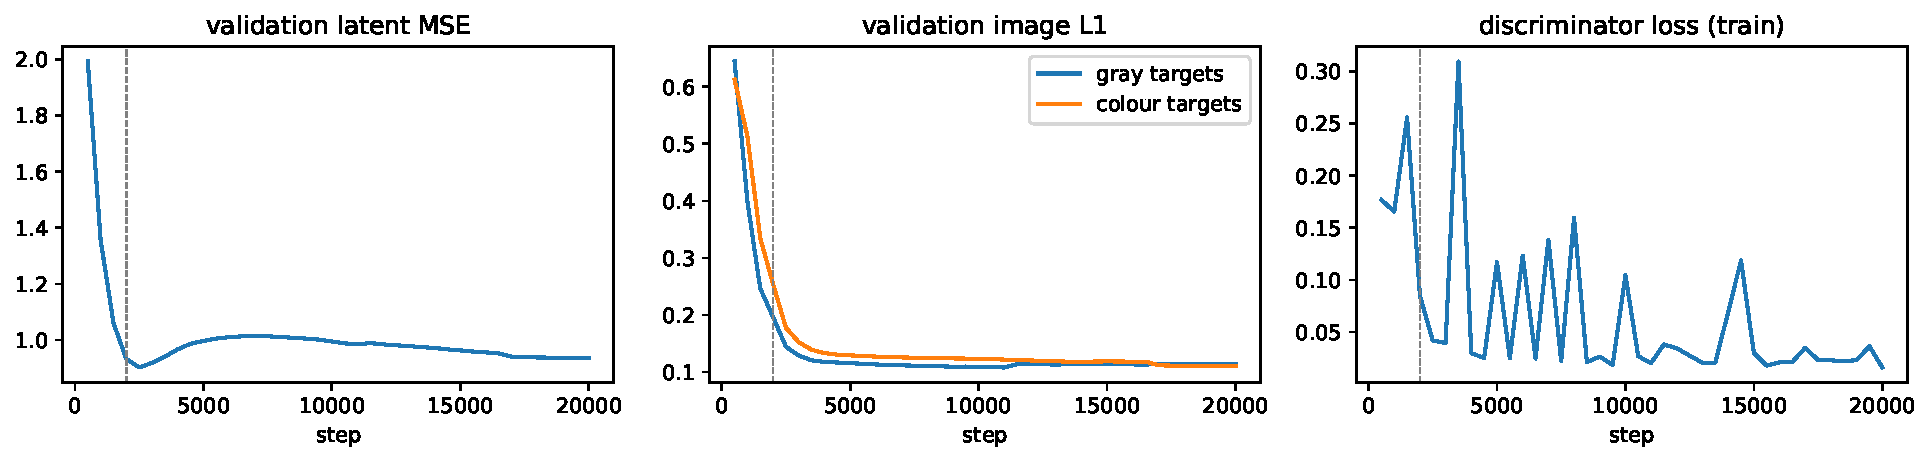
\includegraphics[width=\linewidth]{figures/training_curve_run2.pdf}
\caption{Training of run 2 (validation every 500 steps; dashed line: adversarial terms switched on). The image error
converges by about 5{,}000 steps; the latent error rises slightly once the adversarial terms trade latent accuracy for
realism. The discriminator loss falls to about 0.02, i.e.\ the discriminator dominates, a likely source of the
run-to-run spread. Training curves were logged for run 2 only.}
\label{fig:curve}
\end{figure}

\subsection{Real old photographs}
\label{sec:real}

\begin{table}[t]
\centering
\small
\caption{No-reference quality on the eight real old photographs of BOPBTL's test set (\texttt{test\_images/old}), run 1.
Last row: share of photos on which ours scores better than BOPBTL.}
\label{tab:real}
\begin{tabular}{lccc}
\toprule
 & MUSIQ$\uparrow$ & CLIP-IQA$\uparrow$ & NIQE$\downarrow$ \\
\midrule
Degraded input & 54.11 & \textbf{0.596} & \textbf{3.29} \\
BOPBTL & \textbf{64.89} & 0.515 & 4.72 \\
Ours & 63.56 & 0.444 & 5.24 \\
\midrule
Ours better than BOPBTL & 25\% & 25\% & 25\% \\
\bottomrule
\end{tabular}
\end{table}

We apply both mappings to the eight real old photographs released with BOPBTL, all colour scans. Our mapping raises MUSIQ
well above the input (63.6 vs 54.1) and close to BOPBTL (64.9), but scores lower on CLIP-IQA and NIQE and beats BOPBTL on
only two of the eight photos for each metric (\cref{tab:real}; run 2: 61.9, 0.428, 5.36). CLIP-IQA and NIQE prefer the
unprocessed input to either restoration, which shows how unreliable no-reference metrics are for old photographs; with
eight images the comparison is also small. Qualitatively (\cref{fig:qualitative}) both mappings remove noise and blur
similarly; ours is slightly softer on heavy noise and sometimes brighter. On some near-gray photos with a faint colour
tint, ours produces visible colour patches. We did not conduct a user study; a pairwise preference study on a larger set
of real photographs is left to future work.

\begin{figure*}[p]
\centering
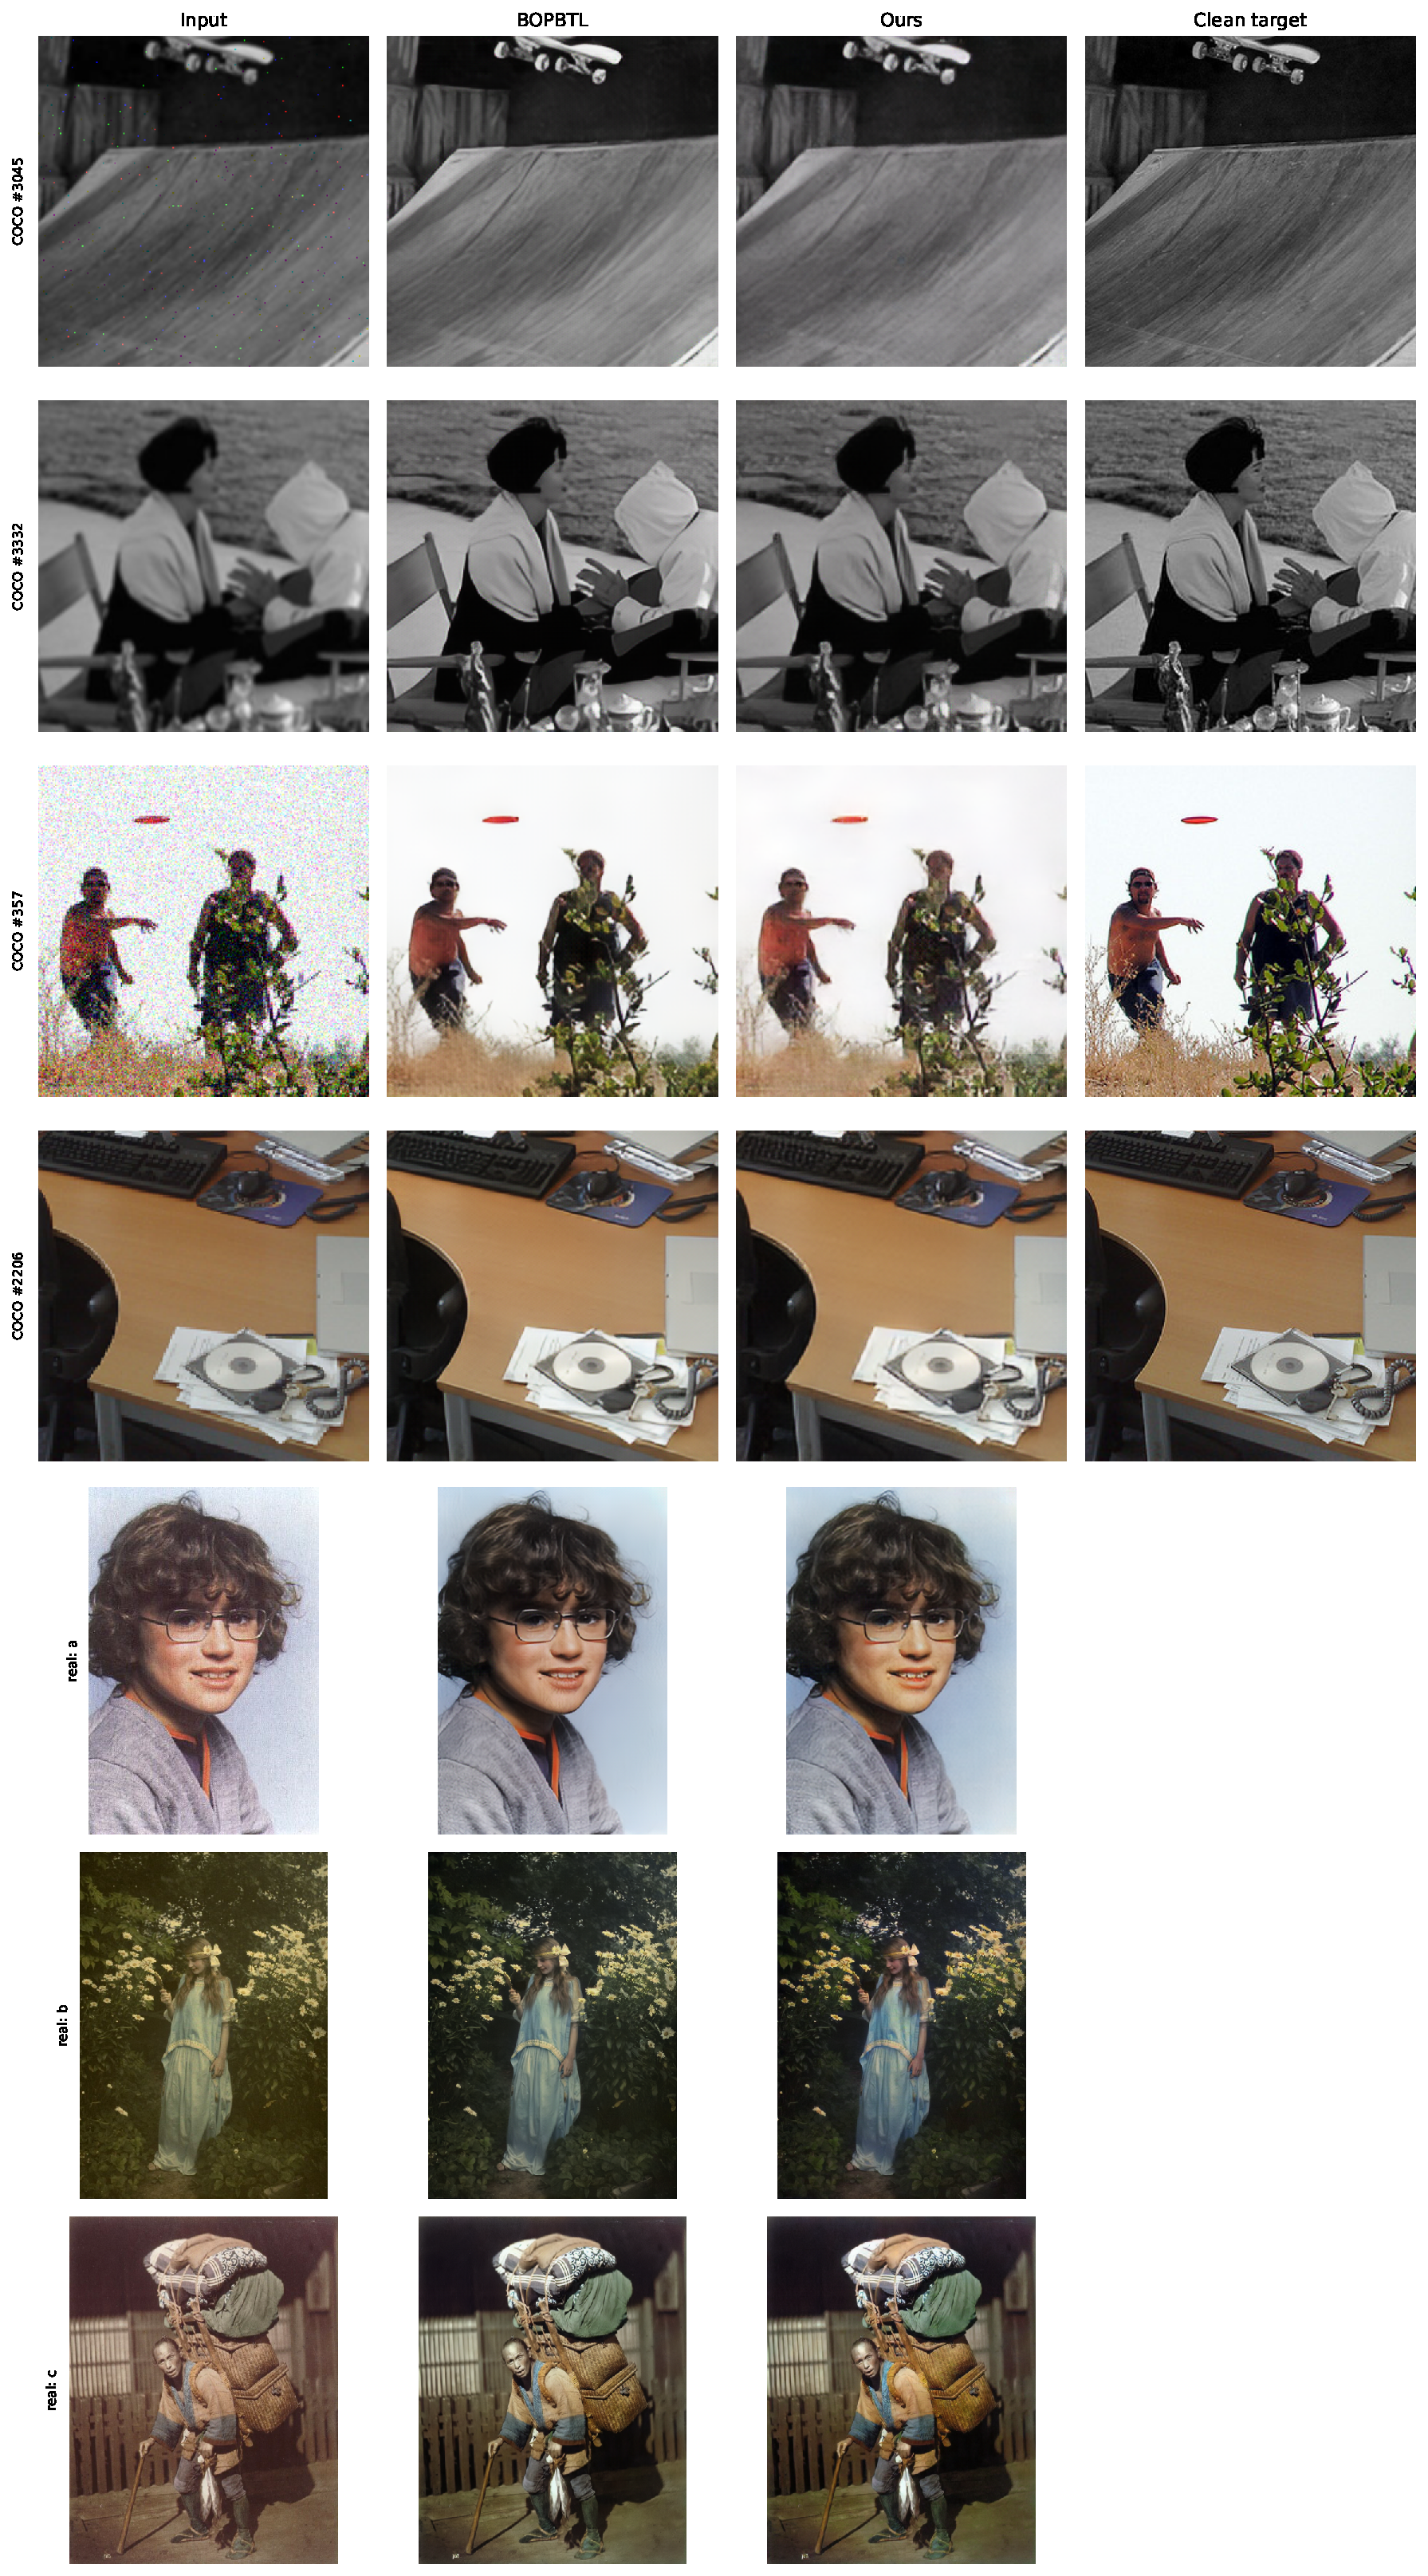
\includegraphics[height=0.86\textheight,keepaspectratio]{figures/qualitative.pdf}
\caption{Qualitative comparison (run 1, no post-processing). Top four rows: COCO benchmark pairs (synthetic degradation)
with the clean target. Bottom three rows: real old photographs (no clean target).}
\label{fig:qualitative}
\end{figure*}

% -----------------------------------------------------------------------------
\section{Limitations}
\label{sec:limits}
Our mapping does not match BOPBTL's quality; its advantage is size and speed, at 68--89\% of BOPBTL's perceptual gain on
synthetic damage. It is less accurate in colour (desaturation, especially of blue) and pixel fidelity, scores lower on
real photos, and can produce colour patches on near-gray photos with a faint tint, a case our test sets do not cover
(the grayscale test pairs are exactly gray). We report two runs of our model and one of each flow configuration; the
spread between our runs is substantial, so the run-1 numbers should be read together with run 2. Our training budget
(batch 8, 20{,}000 steps on one GPU) is far below BOPBTL's (batch 80, 250 epochs on four GPUs). The full-reference
results use synthetic degradations, and the real-photo evaluation uses only eight photographs and no-reference metrics,
without a user study. We address only the global, quality-mode stage of BOPBTL, without scratch removal or face
enhancement.

% -----------------------------------------------------------------------------
\section{Conclusion and future work}
A residual mapping with a third of the parameters and FLOPs of BOPBTL's, trained with the same loss types, keeps most of
its perceptual quality (86--89\% of the LPIPS and KID gain in our better run) and runs two to three times faster; it is
weaker in colour and on real photographs. Flow matching, from which this network originated, contributes nothing in
this setting: a one-step flow is a direct network whose time conditioning folds into normalisation, its optimum equals
direct regression, and in a matched comparison direct training was better on every metric. A flow is the right tool
when no pairing exists. The real gap in old photo restoration is between synthetic and real damage, which BOPBTL bridges
with a latent-space GAN in VAE A. Replacing that alignment with an \emph{unpaired} transport, a flow or Schrödinger
bridge from real old photographs to clean ones with a degradation-invariant content-matching cost, is where we expect
flows to help.

% -----------------------------------------------------------------------------
{\small
\bibliographystyle{ieeetr}
\bibliography{references}
}

\end{document}
